\section{Đề ôn thi giữa kỳ 2 toán 10}
\subsection{Phần trắc nghiệm}
Câu trắc nghiệm nhiều phương án lựa chọn. Học sinh trả lời từ
câu 1 đến câu 12. Mỗi câu hỏi học sinh \textit{chỉ chọn một} phương án.

\Opensolutionfile{ans}[Ans/Dapan]
 
\hienthiloigiaiex
%%%=============EX_1=============%%%
\begin{ex}%[0D3N1-1]%[Dự án đề kiểm tra Toán 10 GHKII NH23-24-Đợt 2-Nắng Đông]%[Đề số 8 - KNTT]
	Biểu thức nào sau đây không là hàm số theo biến $x$?
	\choice
		{$y=\sqrt{x^2-1}$}
		{$y=5x^2-3x+4$}
		{\True $y^4=x^3$}
		{$y=|2x+3|$}
	\loigiai{
		Thay $x=1$ vào $y^4=x^3$ ta được $y^4=1 \Leftrightarrow \hoac{&y=-1\\&y=1.}$\\
		Hay từ một giá trị của $x$ thì có hai giá trị của $y$ nên biểu thức $y^4=x^3$ không phải là hàm số theo biến $x$.
		}
\end{ex}
%%%=============EX_2=============%%%
\begin{ex}%[0D3H2-1]%[Dự án đề kiểm tra Toán 10 GHKII NH23-24-Đợt 2-Nắng Đông]%[Đề số 8 - KNTT]
	Cho hàm số $y=ax^2+bx+c$ có đồ thị như hình vẽ bên dưới. Mệnh đề nào dưới đây là \textbf{đúng}?
	\begin{center}
		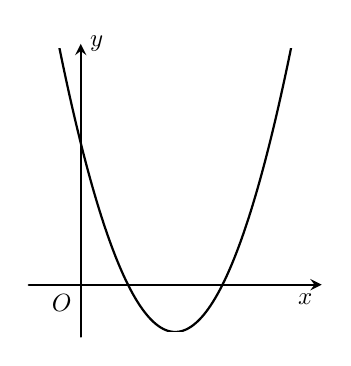
\begin{tikzpicture}[line join=round, line cap=round,>=stealth,thick, scale=0.6]
			\tikzset{every node/.style={scale=0.9}}
			\draw[->] (-1.1,0)--(5.1,0) node[below left] {$x$};
			\draw[->] (0,-1.1)--(0,5.1) node[right] {$y$};
			\draw (0,0) node [below left] {$O$};
			\begin{scope}
				\clip (-1,-1) rectangle (5,5);
				\draw[samples=200,domain=-0.5:4.5,smooth,variable=\x] plot (\x,{(\x)^2-4*(\x)+3});
			\end{scope}
		\end{tikzpicture}
	\end{center}
	\choice
		{$a>0$, $b<0$, $c<0$}
		{$a>0$, $b>0$, $c>0$}
		{\True $a>0$, $b<0$, $c>0$}
		{$a<0$, $b<0$, $c<0$}
	\loigiai{
		Dựa vào hình dáng của đồ thị ta suy ra hệ số $a>0$.\\
		Đồ thị cắt trục tung tại điểm có tung độ dương nên $c>0$.\\
		Parabol có hoành độ đỉnh dương hay $-\dfrac{b}{2a}>0 \Rightarrow b<0$ (vì $a>0$).
		}
\end{ex}
%%%=============EX_3=============%%%
\begin{ex}%[0D3H2-3]%[Dự án đề kiểm tra Toán 10 GHKII NH23-24-Đợt 2-Nắng Đông]%[Đề số 8 - KNTT]
	Cho parabol $(P) \colon y=ax^2+bx+c$ có đồ thị như hình vẽ bên dưới. Giả sử điểm $M(3; m)$ thuộc $(P)$ thì giá trị của $m$ là 
	\begin{center}
		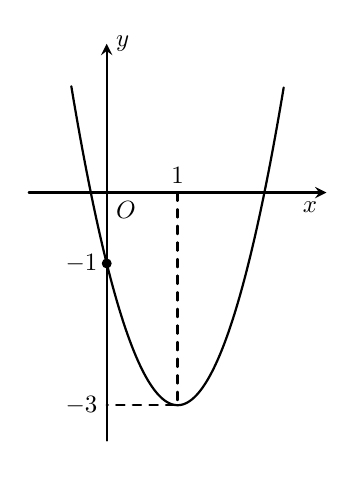
\begin{tikzpicture}[line join=round, line cap=round,>=stealth,thick, scale=0.9]
			\tikzset{every node/.style={scale=0.9}}
			\draw[->] (-1.1,0)--(3.1,0) node[below left] {$x$};
			\draw[->] (0,-3.5)--(0,2.1) node[right] {$y$};
			\draw (0,0) node [below right] {$O$};
			\fill[black] (0,-1)circle(2pt);
			\path (0,-1)node[left]{$-1$};
			\begin{scope}
				\clip (-1,-4) rectangle (3,2);
				\draw[samples=200,domain=-0.5:2.5,smooth,variable=\x] plot (\x,{2*(\x)^2-4*(\x)-1});
				\draw[dashed] (1,0) node[above]{$1$}--(1,-3)--(0,-3) node[left]{$-3$};
			\end{scope}
		\end{tikzpicture}
	\end{center}
	\choice
	{\True $5$}
	{$6$}
	{$7$}
	{$8$}
	\loigiai{
	Dựa vào đồ thị ta thấy $(P)$ có đỉnh $I(1;-3)$ và đi qua điểm $A(0;-1)$ nên ta có hệ phương trình $$\heva{&\dfrac{-b}{2a}=1\\&a+b+c=-3\\&c=-1}\Leftrightarrow \heva{&2a+b=0\\&a+b+c=-3\\&c=-1}\Leftrightarrow \heva{&a=2\\&b=-4\\&c=-1.}$$
	Suy ra $(P) \colon y=2x^2-4x-1$.\\
	Điểm $M(3; m) \in (P) \Rightarrow m=2\cdot 3^2 -4\cdot 3 -1 =5$.
	}
\end{ex}
  %%%============EX_4==============%%%
  \begin{ex}%[0D7H2-1]%[Dự án đề kiểm tra Toán 10 GHKII NH23-24-Đợt 2-Nắng Đông]%[Đề số 8 - KNTT]
  	Tập nghiệm của bất phương trình $x^2+9> 6x$ là
  	\choice
  	{\True $\mathbb{R} \setminus\{3\}$}
  	{$\mathbb{R}$}
  	{$(3;+\infty)$}
  	{$(-\infty; 3)$}
  	\loigiai{
  	Ta có $x^2+9> 6x \Leftrightarrow (x-3)^2>0 \Leftrightarrow x-3 \ne 0 \Leftrightarrow x \ne 3$.\\
  	Vậy tập nghiệm của bất phương trình đã cho là $S=\mathbb{R} \setminus \{3\}$.
  	}
  \end{ex}
  %%%============EX_5==============%%%
  \begin{ex}%[0D7V3-4]%[Dự án đề kiểm tra Toán 10 GHKII NH23-24-Đợt 2-Nắng Đông]%[Đề số 8 - KNTT]
  	Phương trình $\sqrt{x^2-3x+3}+\sqrt{x^2-3x+6}=3$ có tổng tất cả các nghiệm là
  	\choice
  	{$0$}
  	{$1$}
  	{\True $3$}
  	{$5$}
  	\loigiai{
  	Đặt $t=\sqrt{x^2-3x+3},(t\geq 0) \Rightarrow t^2 = x^2-3x+3$.\\
  	Phương trình trở thành
  	$$t+ \sqrt{t^2+3}=3 \Leftrightarrow \sqrt{t^2+3}=3-t \Leftrightarrow \heva{&3-t \geq 0 \\ &t^2+3=(3-t)^2} \Leftrightarrow
  	 \heva{&t \leq 3 \\ &t=1} \Leftrightarrow t=1.$$
  	Với $t=1$ thì $1 = x^2-3x+3 \Leftrightarrow x^2-3x+2=0 \Leftrightarrow \hoac{&x=1\\&x=2.}$\\
  	Vậy tổng tất cả các nghiệm của phương trình là $1+2=3$.
  	}
  \end{ex}
  %%%============EX_6==============%%%
  \begin{ex}%[0D3H1-1]%[Dự án đề kiểm tra Toán 10 GHKII NH23-24-Đợt 2-Nắng Đông]%[Đề số 8 - KNTT]
  	Điều kiện xác định của phương trình $\sqrt{2x-1}=4x+1$ là
  	\choice
  	{$(1;+\infty)$}
  	{\True $\left[\dfrac{1}{2};+\infty\right)$}
  	{$\left[-\dfrac{1}{2};+\infty\right)$}
  	{$\left(-\infty; \dfrac{1}{2}\right]$}
  	\loigiai{
  	Điều kiện xác định của phương trình $\sqrt{2x-1}=4x+1$ là $2x-1 \geq 0 \Leftrightarrow x \geq \dfrac{1}{2}$.\\
  	Vậy tập xác định của hàm số đã cho là $\mathscr{D}=\left[\dfrac{1}{2};+\infty\right)$.
  	}
  \end{ex}
  %%%============EX_7==============%%%
  \begin{ex}%[0H9N1-1]%[Dự án đề kiểm tra Toán 10 GHKII NH23-24-Đợt 2-Nắng Đông]%[Đề số 8 - KNTT]
  	Cho điểm $A(-1;-4)$. Toạ độ điểm $B$ đối xứng với $A$ qua trục hoành là
  	\choice
  	{$(1;-4)$}
  	{\True $(-1; 4)$}
  	{$(1; 4)$}
  	{$(4; 1)$}
  	\loigiai{
  	Điểm $B$ đối xứng với $A(-1;-4)$ qua trục hoành, suy ra $B(-1; 4)$.
  	}
  \end{ex}
  %%%============EX_8==============%%%
  \begin{ex}%[0H9N3-1]%[Dự án đề kiểm tra Toán 10 GHKII NH23-24-Đợt 2-Nắng Đông]%[Đề số 8 - KNTT]
  	Mệnh đề nào sau đây \textbf{sai}?
  	Đường thẳng $d$ được xác định khi ta biết được
  	\choice
  	{\True Một vectơ pháp tuyến hoặc một vectơ chỉ phương của $d$}
  	{Hệ số góc và một điểm thuộc đường thẳng $d$}
  	{Một điểm thuộc $d$ và biết $d$ song song với một đường thẳng cho trước}
  	{Hai điểm phân biệt thuộc $d$}
  	\loigiai{
  	Khi biết một vectơ pháp tuyến hay một vectơ chỉ phương của một đường thẳng thì ta chưa xác định được đường thẳng đó.}
  \end{ex}
   %%%============EX_9==============%%%
  \begin{ex}%[0H9H3-5]%[Dự án đề kiểm tra Toán 10 GHKII NH23-24-Đợt 2-Nắng Đông]%[Đề số 8 - KNTT]
  	Khoảng cách từ điểm $M(4; 5)$ đến đường trung trực của $AB$, với $A(1; 2); B(3; 2)$ bằng
  	\choice
  	{$3$}
  	{\True $2$}
  	{$5$}
  	{$4$}
  	\loigiai{
  	Gọi $d$ là đường trung trực của $AB$ và $I$ là trung điểm của $AB$.\\
  	Khi đó $d$ đi qua điểm $I(2; 2)$ và nhận vectơ $\overrightarrow{AB}=(2; 0)$ làm vectơ pháp tuyến nên phương trình của $d$ là $$2(x-2)+0(y-2)=0 \Leftrightarrow x-2=0.$$
  	Khi đó khoảng cách từ $M(4; 5)$ đến $d$ là $$\mathrm{d}\left(M,d\right)=\dfrac{|4-2|}{\sqrt{1^2+0^2}}=2.$$
  	}
  \end{ex}
  %%%============EX_10==============%%%
  \begin{ex}%[0H9V3-6]%[Dự án đề kiểm tra Toán 10 GHKII NH23-24-Đợt 2-Nắng Đông]%[Đề số 8 - KNTT]
  	Cho $A(1; 1)$, $B(3; 3)$. Tìm $C$ trên $Ox$ sao cho $S_{\triangle ABC}=4$ (đvdt).
  	\choice
  	{$(5; 0)$, $(5; 0)$}
  	{$(-3; 0)$, $(3; 0)$}
  	{\True $(-4; 0)$, $(4; 0)$}
  	{$(-5; 0)$}
  	\loigiai{
  	Đường thẳng $AB$ có phương trình là $y=x$ hay $x-y=0$.\\
  	Ta có điểm $C \in Ox \Rightarrow C(m; 0)$, suy ra $\mathrm{d}\left(C,Ox\right)=\dfrac{|m|}{\sqrt{2}}$.\\
  	Và $\overrightarrow{AB}=(2; 2) \Rightarrow AB=2\sqrt{2}$.\\
  	Khi đó $$S_{\triangle ABC}=\dfrac{1}{2} \cdot AB \cdot \mathrm{d}\left(C,Ox\right) = \dfrac{1}{2} \cdot 2\sqrt{2} \cdot \dfrac{|m|}{\sqrt{2}} = |m|.$$\\
  	Theo đề $$S_{\triangle ABC}=4 \Leftrightarrow |m|=4 \Leftrightarrow  \hoac{&m=4\\&m=-4.}$$
  	Vậy $C(4; 0)$ hoặc $C(-4; 0)$.
  	}
  \end{ex}
  %%%============EX_11==============%%%
  \begin{ex}%[0H9H4-1]%[Dự án đề kiểm tra Toán 10 GHKII NH23-24-Đợt 2-Nắng Đông]%[Đề số 8 - KNTT]
  	Tìm bán kính đường tròn $I(1; 3)$ tiếp xúc $\Delta \colon 3x+2y-7=0$.
  	\choice
  	{$R=\dfrac{\sqrt{13}}{2}$}
  	{$R=\dfrac{3}{\sqrt{13}}$}
  	{\True $R=\dfrac{2}{\sqrt{13}}$}
  	{$R=\dfrac{\sqrt{13}}{3}$}
  	\loigiai{
  	Bán kính $R=\mathrm{d}\left(I,\Delta\right)=\dfrac{|3\cdot 1 + 2\cdot 3 -7 |}{\sqrt{3^2+2^2}}=\dfrac{2}{\sqrt{13}}.$
  	}
  \end{ex}
  %%%============EX_12==============%%%
  \begin{ex}%[0H9H4-2]%[Dự án đề kiểm tra Toán 10 GHKII NH23-24-Đợt 2-Nắng Đông]%[Đề số 8 - KNTT]
  	Trong mặt phẳng toạ độ, đường tròn đi qua ba điểm $A(0; 2)$, $B(-2; 0)$, $C(2; 0)$ có phương trình là
  	\choice
  	{$x^2+y^2=8$}
  	{$x^2+y^2+2x+4=0$}
  	{$x^2+y^2-2x-8=0$}
  	{\True $x^2+y^2-4=0$}
  	\loigiai{
  	Gọi phương trình đường tròn $(C)$ cần tìm có dạng $x^2+y^2-2ax - 2by + c=0$, điều kiện $a^2+b^2-c>0$.\\
  	Đường tròn $(C)$ đi qua ba điểm $A(0; 2)$, $B(-2; 0)$, $C(2; 0)$ nên ta có hệ phương trình $$\heva{&-4b+c=-4\\&4a+c=-4\\&-4a+c=-4} \Leftrightarrow \heva{&a=0\\&b=0\\&c=-4.}\text{(thỏa điều kiện)}$$
  	Vậy phương trình của $(C)$ là $x^2+y^2-4=0$.
  	}
  \end{ex}
   
\Closesolutionfile{ans}
\bangdapan{Dapan}


\subsection{Câu trắc nghiệm đúng sai}
Học sinh trả lời từ câu 1 đến câu 4.
Trong mỗi ý \circlenum{A}, \circlenum{B}, \circlenum{C} và \circlenum{D} ở mỗi câu, học sinh chọn đúng hoặc sai.
\setcounter{ex}{0}
\LGexTF
\Opensolutionfile{ansbook}[ansbook/DapanDS08]
\Opensolutionfile{ans}[Ans/DapanT08]
%%%============EX_1==============%%%
\begin{ex}%[0D3H2-3]%[Dự án đề kiểm tra Toán khối 10 GHKII NH23-24-Dot 2-Đoàn Minh Tâm]%[Deso08-KNTT]
	\immini{Cho hàm số $y=-x^2-2$. Khi đó
		\choiceTF
		{\True Đồ thị của hàm số có đỉnh $I(0 ;-2)$}
		{Đồ thị của hàm số có trục đối xứng là đường thẳng $x=1$}
		{\True Đồ thị của hàm số giao điểm với trục $O y$ là $I(0 ;-2)$}
		{\True Đồ thị như Hình 1}}{
		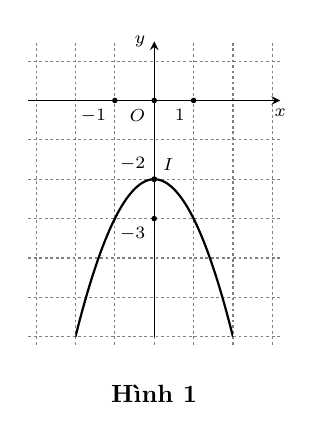
\begin{tikzpicture}[>=stealth,x=1cm,y=1cm,scale=0.5]
			\def\a{-1} % Hệ số a phải khác 0
			\def\b{0}
			\def\c{-2}
			\draw[color=gray,dash pattern=on 1pt off 1pt,xstep=1.0cm,ystep=1.0cm] (-3.2,-6.2) grid (3.2,1.5);
			\draw[->] (-3.2,0) -- (3.2,0) node[below] {\scriptsize $x$};
			\draw[->] (0,-6) -- (0,1.5) node[left] {\scriptsize $y$};
			\draw (0,0)node[below left]{\scriptsize $O$};
			\pgfmathsetmacro\xdinh{-(\b)/2*(\a)}
			\pgfmathsetmacro\ydinh{(4*(\a)*(\c)-(\b)^2)/(4*(\a))}
			\fill (0,0) circle(2pt) ;
			\fill (\xdinh,\ydinh)node[above right]{\scriptsize $I$}circle(2pt) ;
			\fill (-1,0) node[below left]{\scriptsize $-1$} circle(2pt) ;
			\fill (1,0) node[below left]{\scriptsize $1$} circle(2pt) ;
			\fill (0,-2) node[above left]{\scriptsize $-2$} circle(2pt) ;
			\fill (0,-3) node[below left]{\scriptsize $-3$} circle(2pt) ;
			\path (0,-7) node[below]{\textbf{Hình 1}};
			\clip (-2,-6)rectangle(2,1);
			\draw[thick,samples=150,smooth,domain=-5:5] plot(\x,{\a*(\x)^2+(\b)*\x+(\c)});
		\end{tikzpicture}
	}
	\loigiai{
		\immini{
			\begin{itemize}
				\item Tọa độ đỉnh của đồ thị hàm số là $\heva{&x=-\dfrac{0}{2\cdot(-1)}=0\\&y=-0^2-2=-2.}$\\
				Vậy đỉnh của đồ thi hàm số là $I(0;-2)$.
				\item Đồ thị hàm số có trục đối xứng là $x=-\dfrac{0}{2\cdot(-1)}=0$.
				\item Do tọa độ đỉnh của đồ thị hàm số là $I(0;-2)$ nên giao điểm với trục $Oy$ là $I(0;-2)$.
				\item Ta có đỉnh của đồ thị hàm số là $I(0;-2)$.\\
				Đồ thị hàm số có trục đối xứng là $Oy$.\\
				Bảng giá trị của hàm số là
				\begin{center}
					\renewcommand\arraystretch{1.8} %độ rộng của hàng
					\begin{tabular}{c|ccccccccc}
						$x$&$-1$&&$0$&&$1$\\
						\hline
						$y = -x^2-2$&$-3$&&$-2$&&$-3$
					\end{tabular}
				\end{center}
				Nên đồ thị hàm số như Hình 1.
		\end{itemize}}{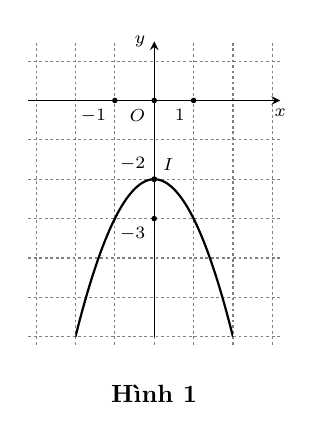
\begin{tikzpicture}[>=stealth,x=1cm,y=1cm,scale=0.5]
				\def\a{-1} % Hệ số a phải khác 0
				\def\b{0}
				\def\c{-2}
				\draw[color=gray,dash pattern=on 1pt off 1pt,xstep=1.0cm,ystep=1.0cm] (-3.2,-6.2) grid (3.2,1.5);
				\draw[->] (-3.2,0) -- (3.2,0) node[below] {\scriptsize $x$};
				\draw[->] (0,-6) -- (0,1.5) node[left] {\scriptsize $y$};
				\draw (0,0)node[below left]{\scriptsize $O$};
				\pgfmathsetmacro\xdinh{-(\b)/2*(\a)}
				\pgfmathsetmacro\ydinh{(4*(\a)*(\c)-(\b)^2)/(4*(\a))}
				\fill (0,0) circle(2pt) ;
				\fill (\xdinh,\ydinh)node[above right]{\scriptsize $I$}circle(2pt) ;
				\fill (-1,0) node[below left]{\scriptsize $-1$} circle(2pt) ;
				\fill (1,0) node[below left]{\scriptsize $1$} circle(2pt) ;
				\fill (0,-2) node[above left]{\scriptsize $-2$} circle(2pt) ;
				\fill (0,-3) node[below left]{\scriptsize $-3$} circle(2pt) ;
				\path (0,-7) node[below]{\textbf{Hình 1}};
				\clip (-2,-6)rectangle(2,1);
				\draw[thick,samples=150,smooth,domain=-5:5] plot(\x,{\a*(\x)^2+(\b)*\x+(\c)});
		\end{tikzpicture}}
	}
\end{ex}

%%%============EX_2==============%%%
\begin{ex}%[0D7H3-1]%[Dự án đề kiểm tra Toán khối 10 GHKII NH23-24-Dot 2-Đoàn Minh Tâm]%[Deso08-KNTT]
	Cho phương trình $\sqrt{2 x^2+5}=\sqrt{x^2-x+11}\quad(*)$. Khi đó
	\choiceTF
	{Điều kiện $x \geq 0$}
	{\True Bình phương $2$ vế phương trình $(*)$ ta được $x^2+x-6=0$}
	{Phương trình $(*)$ có 1 nghiệm}
	{Giả sử $x_1$, $x_2$ $\left(x_1<x_2\right)$ là nghiệm của phương trình $(*)$ khi đó $x_1-2 x_2=7$}
	\loigiai{ \\
		Ta có $\sqrt{2 x^2+5}=\sqrt{x^2-x+11}\Rightarrow 2 x^2+5=x^2-x+11 \Rightarrow x^2+x-6=0 \Rightarrow \hoac{&x=2\\&x=-3.}$\\
		Thử lại ta nhận $x=2$ và $x=-3$ là nghiệm.
		\begin{itemize}
			\item Điều kiện $\heva{&2x^2+5 \ge 0 \\&x^2-x+11\ge 0}\Leftrightarrow x \in \mathbb{R}$.
			\item Bình phương $2$ vế phương trình $(*)$ ta được $2 x^2+5=x^2-x+11 \Leftrightarrow x^2+x-6=0$.
			\item Ta có phương trình $(*)$ có 2 nghiệm là $x=2$ và $x=-3$.
			\item Ta có $x_1=-3$, $x_2=2$ nên $x_1-2x_2=-3-2\cdot 2 =-7$.
		\end{itemize}
	}
\end{ex}

%%%============EX_3==============%%%
\begin{ex}%[0H9H3-2]%[Dự án đề kiểm tra Toán khối 10 GHKII NH23-24-Dot 2-Đoàn Minh Tâm]%[Deso08-KNTT]
	Chuyển động của vật thể $M$ được thể hiện trên mặt phẳng toạ độ $O x y$. Vật thể $M$ khởi hành từ điểm $A(5 ; 3)$ và chuyển động thẳng đều với vectơ vận tốc là $\overrightarrow{v}(1 ; 2)$. Khi đó
	\choiceTF
	{\True Vectơ chỉ phương của đường thẳng biểu diễn chuyển động của vật thể là $\overrightarrow{v}(1 ; 2)$}
	{Vật thể $M$ chuyển động trên đường thẳng $2 x-3 y-1=0$}
	{\True Toạ độ của vật thể $M$ tại thời điểm $t$ $(t>0)$ tính từ khi khởi hành là $\heva{&x=5+t \\ &y=3+2 t}$}
	{\True Khi $t=5$ thì vật thể $M$ chuyển động được quãng đường dài bằng $5 \sqrt{5}$}
	\loigiai{
		\begin{itemize}
			\item Do vật chuyển động thẳng đều với vectơ vận tốc là $\overrightarrow{v}(1 ; 2)$ nên vectơ chỉ phương của đường thẳng biểu diễn chuyển động của vật thể là $\overrightarrow{v}(1 ; 2)$.
			\item Ta có vật thể $M$ chuyển động với quỹ đạo là đường thẳng $d$ đi qua $A(5;3)$ và nhận $\overrightarrow{v}(1 ; 2)$ làm vectơ chỉ phương nên nhận $\overrightarrow{n}=(2;-1)$ làm vectơ pháp tuyến.\\
			Khi đó phương trình tổng quát của đường thẳng $d$ là
			$$2(x-5)-1(y-3)=0\Leftrightarrow 2x-y-7=0.$$
			\item Phương trình tham số của đường thẳng $d$ là $\heva{&x=5+t\\&3+2t.}$\\
			Vậy toạ độ của vật thể $M$ tại thời điểm $t$ $(t>0)$ tính từ khi khởi hành là $\heva{&x=5+t \\ &y=3+2 t.}$
			\item Khi $t=5$, vật thể $M$ chuyển động đến vị trí là $\heva{&x=5+5 \\ &y=3+2 \cdot 5} \Leftrightarrow \heva{&x=10\\&y=13}\Rightarrow N(10;13)$.\\
			Vậy quãng đường di chuyển của vật là $MN=\sqrt{(10-5)^2+(13-3)^2}=5\sqrt{5}$.
		\end{itemize}
		
	}
\end{ex}

%%%============EX_4==============%%%
\begin{ex}%[0H9H4-2]%[Dự án đề kiểm tra Toán khối 10 GHKII NH23-24-Dot 2-Đoàn Minh Tâm]%[Deso08-KNTT]
	Đường tròn $(C)$ đi qua hai điểm $A(2 ; 3)$, $B(-1 ; 1)$ có tâm thuộc $\Delta\colon x-3 y-11=0$. Khi đó
	\choiceTF
	{Tâm của đường tròn $(C)$ là $I\left(7 ;-\dfrac{4}{3}\right)$}
	{\True Điểm $O(0 ; 0)$ nằm bên trong đường tròn $(C)$}
	{Đường kính của đường tròn $(C)$ bằng $65$}
	{\True Đường tròn  $(C)$ đi qua điểm $N(0;2)$}
	\loigiai{\\
		Gọi phương trình đường tròn $(C)$ là $x^2+y^2-2ax-2by+c=0$, có tâm là $I(a;b)$.\\
		Do $I \in \Delta \Rightarrow a-3b-11=0 \Leftrightarrow a-3b=11.\qquad (1)$\\
		Do $A(2;3)$ và $B(-1;1) \in (C)$ nên
		$$\heva{&2^2+3^2-2a\cdot 2 -2b\cdot 3+c=0\\&(-1)^2+1^2-2a\cdot(-1)-2b\cdot 1+c=0}\Leftrightarrow \heva{&-4a-6b+c=-13&(2)\\&2a-2b+c=-2&(3).}$$
		Từ $(1)$, $(2)$ và $(3)$ ta được hệ $\heva{&a-3b=11\\&-4a-6b+c=-13\\&2a-2b+c=-2}\Leftrightarrow\heva{&a=\dfrac{7}{2}\\&b=-\dfrac{5}{2}\\&c=-14.}$\\
		Vậy phương trình đường tròn $(C)$ là $x^2+y^2-7x+5y-14=0$.\\
		Đường tròn $(C)$ có $\heva{&\text{có tâm }I\left(\dfrac{7}{2};-\dfrac{5}{2}\right)\\&\text{bán kính }R=\sqrt{\left(\dfrac{7}{2}\right)^2+\left(-\dfrac{5}{2}\right)^2-(-14)}=\dfrac{\sqrt{130}}{2}.}$
		\begin{itemize}
			\item Tâm của đường tròn là $I\left(\dfrac{7}{2};-\dfrac{5}{2}\right)$.
			\item Ta có $OI=\sqrt{\left(\dfrac{7}{2}\right)^2+\left(-\dfrac{5}{2}\right)^2}=\dfrac{\sqrt{74}}{2}<\dfrac{\sqrt{130}}{2}$ nên điểm $O(0;0)$ nằm bên trong $(C)$.
			\item Đường kính của đường tròn $(C)$ là $2R=2\cdot \dfrac{\sqrt{130}}{2}=\sqrt{130}$.
			\item Thay $N(0;2)$ vào $(C)$, ta có $0^2+2^2-7\cdot 0 +5\cdot 2-14=0$ nên $N \in (C)$.
		\end{itemize}
	}
\end{ex}

\Closesolutionfile{ans}
\Closesolutionfile{ansbook}

\begin{center}
	\textbf{\textsf{BẢNG ĐÁP ÁN ĐÚNG SAI}}
\end{center}
\input{Ansbook/DapanDS08}


\subsection{Phần tự luận}

\hienthiloigiaibt
%%==========Câu 1
\begin{bt}%[0D3H2-6]
	Cổng Arch tại thành phố St Louis của Mỹ có hình dạng là một parabol. Biết khoảng cách giữa hai chân cổng bằng $162$ m. Trên thành cổng, tại vị trí có độ cao $43$ m so với mặt đất, người ta thả một sợi dây chạm đất. Vị trí chạm đất của đầu sợi dây này cách chân cổng $A$ một đoạn $10$ m. Giả sử các số liệu trên là chính xác. Hãy tính độ cao của cổng Arch.
	\loigiai{
		Chọn hệ trục tọa độ $Oxy$ sao cho một chân cổng $A$ đặt tại gốc tọa độ, chân còn lại đặt trên tia $Ox$. Ta có hình vẽ sau
		\begin{center}
			\begin{tikzpicture}[scale=.8,>=stealth]
				\draw[->,>=stealth] (-3,0) -- (6.5,0);
				\draw[->,>=stealth] (-1.1622,-2) -- (-1.1622,6);
				% Vẽ 2 trục, điền các số lên trục
				\draw[<->,>=stealth] (-1.1622,-0.3) -- (0,-0.3); \node at (-0.5811,-0.3) [below] {10 m};
				\node at (2,0.3) {162 m};
				\draw[thick,samples=100,domain=-1.1622:5.1622, line width=1pt,color=blue] 
				plot(\x,{-0.5*(\x)^2+2*(\x)+3});
				% Vẽ thêm mấy cái râu ria
				\draw[dashed] (0,3) -- (0,0);\node at (0,1.5) [right] {43 m};
				\draw (-1.1622,0)--(5.1622,0);
				\def\a{1.5}\def\r{2}
				\node at (-1.1622,0) [above left]{{$A$}};
				\node at (-1.1622,6) [above]{{$y$}};
				\node at (6.5,0) [right]{{$x$}};
				\node at (5.1622,0) [above right]{{$B$}};
				\node at (0,3) [left] {$M$};
				\draw [fill=black] (0.,3.) circle (2.0pt);
				\draw [fill=black] (-1.1622,0) circle (2.0pt);
				\draw [fill=black] (5.1622,0) circle (2.0pt);
			\end{tikzpicture}
		\end{center}
		Parabol $(P)\colon y=ax^2+bx+c$ đi qua điểm $A(0;0)$, $B(162;0)$, $M(10;43)$ nên ta có\\ 
		$\heva{& c=0\\& 162^2a+162b+c=0\\& 10^2+10b+c=43}\Leftrightarrow\heva{& c=0\\& a=-\dfrac{43}{1520}\\& b=\dfrac{3483}{760}}\Rightarrow\left(P\right)\colon y=-\dfrac{43}{1520}x^2+\dfrac{3483}{760}x.$\\
		Do đó chiều cao của cổng là $h=-\dfrac{\Delta}{4a}=-\dfrac{b^{2}-4ac}{4a} \approx 185{,}6$ m.
	}
\end{bt}

%%==========Câu 2
\begin{bt}%[0D3H1-7]
	Bảng giá trị điện sinh hoạt được mô tả như sau
	\begin{center}
		\begin{tabular}{|c|c|}
			\hline
			Mức điện tiêu thụ	& Giá bán điện (đồng/kWh)\\
			\hline
			Bậc $1$ (từ $0$ đến $50$ kWh)	& $1678$\\
			\hline
			Bậc $2$ (từ $50$ đến $100$ kWh)	& $1734$\\
			\hline
			Bậc $3$ (từ $100$ đến $200$ kWh)	& $2014$\\
			\hline
			Bậc $4$ (từ $200$ đến $300$ kWh)	& $2536$\\
			\hline
			Bậc $5$ (từ $300$ đến $400$ kWh)	& $2834$\\
			\hline
			Bậc $6$ (từ $400$ kWh trở lên)	& $2927$\\
			\hline
		\end{tabular}\\
		(Theo Tập đoàn Điện Lực Việt Nam ngày $28/10/2021$)
	\end{center}
	Nếu một hộ gia đình phải trả số tiền dùng trong tháng là $767300$ đồng thì số kWh điện (số điện) tiêu thụ của hộ gia đình trong tháng đó là bao nhiêu?
	\loigiai{
		Gọi $x$ là lượng điện tiêu thụ (đơn vị kWh) và $y$ là số tiền phải trả tương ứng (đơn vị đồng).\\
		Theo đề bài ta có công thức mô tả sự phụ thuộc $y$ vào $x$ là 
		\[y=50\cdot 1678+50\cdot 1734+100\cdot 2014+100\cdot 2536+(x-300)\cdot 2834.\]
		Suy ra $y=2834x-224600$. Do đó khi gia đình phải trả số tiền là $767300$ đồng thì số kWh điện tiêu thụ của gia đình trong tháng đó là $767300=2834x-224600$. Suy ra $x=350$ kWh.
	}
\end{bt}

%%==========Câu 3
\begin{bt}%[0D7H3-3]
	Tập hợp tất cả tham số $m$ để phương trình $\sqrt{2x^2-6x+m}=x-1$ có $2$ nghiệm phân biệt là nửa khoảng $\left[a;b\right)$ với $a; b \in \mathbb{Z}$. Tính diện tích một tam giác vuông có cạnh huyền bằng $b$ và một cạnh góc vuông bằng $a$
	\loigiai{
		Phương trình đã cho tương đương\\
		$\heva{& x-1\ge 0\\& 2x^2-6x+m=\left(x-1\right)^2}\Leftrightarrow\heva{& x\ge 1\\& x^2-4x+m-1=0\;(*)}$\\
		Phương trình đã cho có hai nghiệm phân biệt $\Leftrightarrow (*)$ có $2$ nghiệm phân biệt $\ge 1$.
		\allowdisplaybreaks
		\begin{eqnarray*}
			&\Leftrightarrow&\heva{& \Delta =16-4\left(m-1\right)>0\\& x_2>x_1=\dfrac{4-\sqrt{\Delta}}{2}\ge 1}
			\Leftrightarrow\heva{& 20-4m>0\\& \dfrac{4-\sqrt{20-4m}}{2}\ge 1}\\
			&\Leftrightarrow&\heva{& m<5\\& \sqrt{20-4m}\le 2}\Leftrightarrow\heva{& m<5\\& m\ge 4}\\
			&\Leftrightarrow& 4\le m<5.
		\end{eqnarray*}
		Ta có $a=4$, $b=5$, cạnh góc vuông tương ứng còn lại tam giác là $\sqrt{5^2-4^2}=3$.\\
		Diện tích tam giác đó bằng $\dfrac{1}{2}\cdot 4\cdot 4=6$.
	}
\end{bt}


%%==========Câu 4
\begin{bt}%[0H9H2-1]
	Cho tam giác $ABC$ có các đỉnh $A(1;1), B(2;4), C(10;-2)$. Tính diện tích tam giác $ABC$
	%\shortans[3]{$\dfrac{30}{2}$}
	\loigiai{
		Ta có $\overrightarrow{AB}=(1;3)$, $\overrightarrow{AC}=(9;-3)$.\\
		$\overrightarrow{AB}\cdot \overrightarrow{AC}=1\cdot 9+3(-3)=0 \Rightarrow \overrightarrow{AB} \perp \overrightarrow{AC}$.
		Vậy tam giác $ABC$ vuông tại $A$.\\
		Ta có $AB=\sqrt{1^2+3^2}=\sqrt{10}$, $AC=\sqrt{9^2+(-3)^2}=3 \sqrt{10}$.\\
		Diện tích tam giác $ABC$ là $S_{\triangle ABC}=\dfrac{1}{2} AB\cdot AC=\dfrac{1}{2}\cdot \sqrt{10}\cdot 3 \sqrt{10}=\dfrac{30}{2}$.
	}
\end{bt}

%%==========Câu 5
\begin{bt}%[0H9H3-2]
	Viết phương trình đường thẳng $\Delta$ đi qua $M$ và cách đều các điểm $P$, $Q$ với $M(2;5)$, $P(-1;2)$, $Q(5;4)$.
	%\shortans[3]{$d\colon x-3y+13=0$; $d\colon x=2$.}
	\loigiai{
		Gọi $\overrightarrow{n}=(a;b)$ là vectơ pháp tuyến của đường thẳng $d$ cần tìm.\\
		Ta có $d$ qua $M(2;5)$ nên phương trình  $d$ có dạng $a(x-2)+b(y-5)=0$.\\
		Ta có \begin{eqnarray*}
			\mathrm{d}(P, d)=\mathrm{d}(Q, d)&\Leftrightarrow&\dfrac{|-3a- 3b|}{\sqrt{a^2+b^2}}=\dfrac{|3 a- b|}{\sqrt{a^2+b^2}}\\
			&\Leftrightarrow& \hoac{&-3a-3b=3a-b\\&3a+3b=3a-b}\\
			&\Leftrightarrow& \hoac{&b=-3a\\&b=0.}
		\end{eqnarray*}
		Với $b=-3a$, chọn $a=1$ suy ra $b=-3$.\\
		Với $b=0$, ta chọn $a=1$.\\
		Vậy có hai phương trình đường thẳng thỏa mãn đề bài là $d\colon x-3y+13=0$; $d\colon x=2$.
	}
\end{bt}

%%==========Câu 6
\begin{bt}%[0H9V4-3]
	Trong mặt phẳng $Oxy$, cho đường tròn $(C)\colon x^2+y^2+2x-6y+5=0$. Viết phương trình tiếp tuyến của $(C)$ song song với đường thẳng $d\colon x+2y-15=0$.
	%\shortans[3]{$x+2y=0$ và $x+2y-10=0$.}
	\loigiai{
		Đường tròn $(C)$ có tâm $I(-1;3)$ và bán kính $R=\sqrt{1+9-5}=\sqrt{5}$.\\
		Tiếp tuyến $\Delta \parallel d$ nên phương trình $\Delta$ có dạng $x+2y+m=0;\,m \neq-15$.\\
		Ta có $\Delta$ là tiếp tuyến của $(C)$ khi và chỉ khi 
		\begin{eqnarray*}
			\mathrm{d}(I,\Delta)=R&\Leftrightarrow& \dfrac{|-1+6+m|}{\sqrt{1+4}}=\sqrt{5}\\  &\Leftrightarrow& |m+5|=5\\
			&\Leftrightarrow&\hoac{&m+5=-5\\&m+5=5}\\
			&\Leftrightarrow&\hoac{&m=-10\\&m=0.}
		\end{eqnarray*}
		Đối chiếu với điều kiện, ta có hai phương trình tiếp tuyến của $(C)$ là $x+2y=0$ và $x+2y-10=0$.
	}
\end{bt}
